\documentclass[tikz,border=10pt]{standalone}
\usepackage{tikz}
\usetikzlibrary{positioning}
\usepackage{tikz-feynman}
\begin{document}

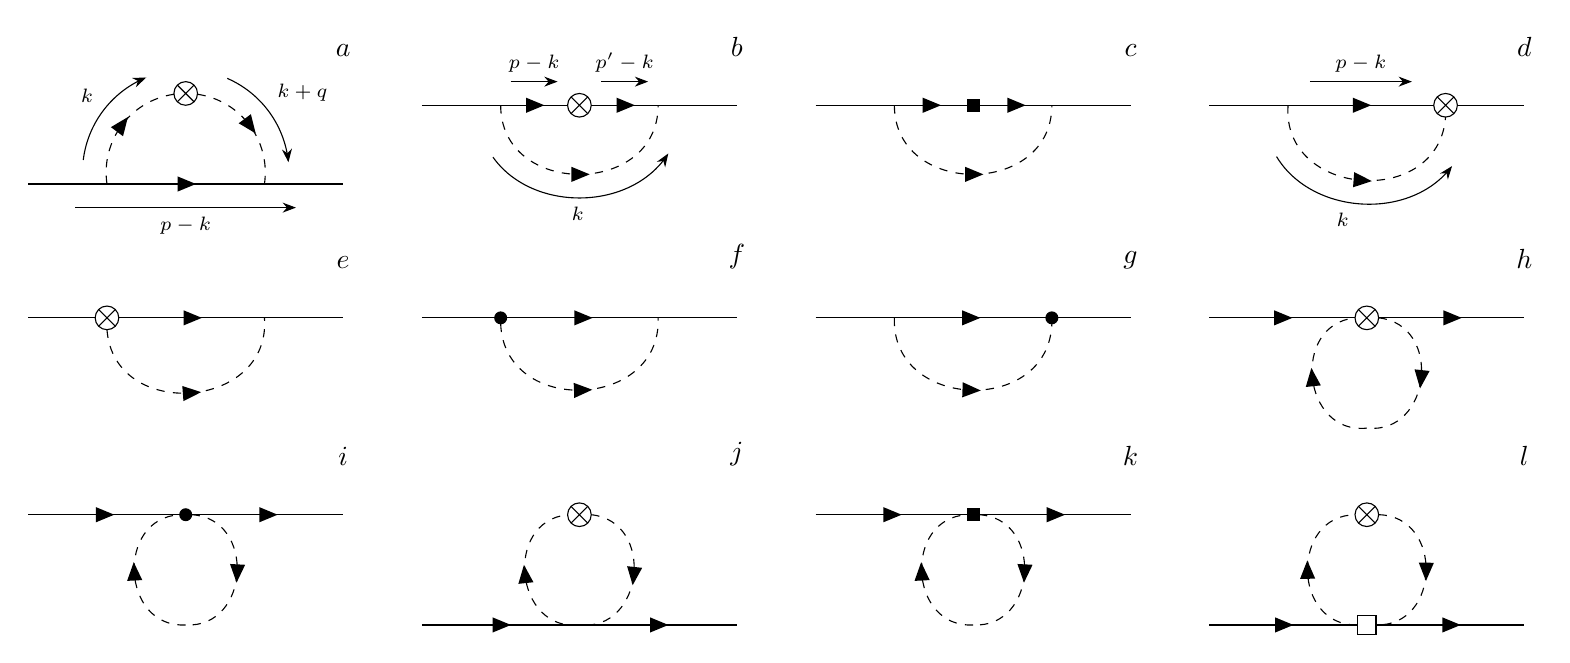
\begin{tikzpicture}
	\begin{feynman}
		%% fig a
		\vertex (a1) at (0,0);
		\vertex[right =1cm  of a1] (a2);
		\vertex[right =2cm  of a1] (a3);
		\vertex[right =3cm  of a1] (a4);
		\vertex[right =4cm  of a1] (a5);
		\vertex[above =1cm of a3,crossed dot] (a6){};
		\node[above =1.5cm  of a5] {$a$};
		%% fig b
		\vertex[above right =1cm and 5cm of a1] (b1);
		\vertex[right =1cm  of b1] (b2);
		\vertex[right =2cm  of b1,crossed dot,anchor=center] (b3){};
		\vertex[right =3cm  of b1] (b4);
		\vertex[right =4cm  of b1] (b5);
		\node[above =0.5 of b5] {$b$};
		%% fig c
		\vertex[above right =1cm and 10cm of a1] (c1);
		\vertex[right =1cm  of c1] (c2);
		\vertex[right =2cm  of c1,square dot,anchor=center] (c3){};
		\vertex[right =3cm  of c1] (c4);
		\vertex[right =4cm  of c1] (c5);
		\node[above =0.5 of c5] {$c$};
		%% fig d
		\vertex[above right =1cm and 15cm of a1] (d1);
		\vertex[right =1cm  of d1] (d2);
		\vertex[right =2cm  of d1] (d3);
		\vertex[right =3cm  of d1,crossed dot,anchor=center] (d4){};
		\vertex[right =4cm  of d1] (d5);
		\node[above =0.5 cm  of d5] {$d$};
		%% fig e
		\vertex[below right =1.7 cm and 0 cm of a1] (e1);
		\vertex[right =1cm  of e1,crossed dot,anchor=center] (e2){};
		\vertex[right =2cm  of e1] (e3);
		\vertex[right =3cm  of e1] (e4);
		\vertex[right =4cm  of e1] (e5);
		\node[above =0.5cm of e5] {$e$};
		%% fig f
		\vertex[below right =0 cm and 5 cm of e1] (f1);
		\vertex[right =1cm  of f1, dot,anchor=center] (f2){};
		\vertex[right =2cm  of f1] (f3);
		\vertex[right =3cm  of f1] (f4);
		\vertex[right =4cm  of f1] (f5);
		\node[above =0.5cm  of f5] {$f$};
		%% fig g
		\vertex[below right =0 cm and 10 cm of e1] (g1);
		\vertex[right =1cm  of g1] (g2);
		\vertex[right =2cm  of g1] (g3);
		\vertex[right =3cm  of g1, dot,anchor=center] (g4){};
		\vertex[right =4cm  of g1] (g5);
		\node[above =0.5cm  of g5] {$g$};
		%% fig h
		\vertex[below right =0 cm and 15 cm of e1] (h1);
		\vertex[right =1cm  of h1] (h2);
		\vertex[right =2cm  of h1, crossed dot,anchor=center] (h3){};
		\vertex[right =3cm  of h1] (h4);
		\vertex[right =4cm  of h1] (h5);
		\vertex[above =-1.4cm  of h3] (h6);
		\node[above =0.5cm  of h5] {$h$};
		%% fig i
		\vertex[below right =2.5 cm and 0 cm of e1] (i1);
		\vertex[right =1cm  of i1] (i2);
		\vertex[right =2cm  of i1,  dot,anchor=center] (i3){};
		\vertex[right =3cm  of i1] (i4);
		\vertex[right =4cm  of i1] (i5);
		\vertex[above =-1.4cm  of i3] (i6);
		\node[above =0.5 cm  of i5] {$i$};
		%% fig j
		\vertex[below right =1.4 cm and 5 cm of i1] (j1);
		\vertex[right =1cm  of j1] (j2);
		\vertex[right =2cm  of j1] (j3);
		\vertex[right =3cm  of j1] (j4);
		\vertex[right =4cm  of j1] (j5);
		\vertex[above =1.4 cm  of j3, crossed dot,anchor=center] (j6){};
		\node[above =1.9 cm  of j5] {$j$};
		%% fig k
		\vertex[below right =0 cm and 10 cm of i1] (k1);
		\vertex[right =1cm  of k1] (k2);
		\vertex[right =2cm  of k1, square  dot,anchor=center] (k3){};
		\vertex[right =3cm  of k1] (k4);
		\vertex[right =4cm  of k1] (k5);
		\vertex[above =-1.4cm  of k3] (k6);
		\node[above =0.5 cm  of k5] {$k$};
		%% fig l
		\vertex[below right =1.4 cm and 15 cm of i1] (l1);
		\vertex[right =1cm  of l1] (l2);
		\vertex[right =2cm  of l1,shape=rectangle, minimum size=0.1cm,draw,anchor=center] (l3){};
		\vertex[right =3cm  of l1] (l4);
		\vertex[right =4cm  of l1] (l5);
		\vertex[above =1.4cm  of l3, crossed dot, anchor=center] (l6){};
		\node[above =1.9  cm  of l5] {$l$};
		% 对各个顶点连线
		\diagram*{
		{ [edge= fermion]
		(a1) --[momentum'={\scriptsize \(p-k\)}]  (a5),
		(b2) --[momentum={\scriptsize \(p-k\)}]  (b3)-- [momentum={\scriptsize \(p^{\prime}-k\)}] (b4),
		(c2) --  (c3)--  (c4),
		(d2) -- [momentum={\scriptsize \(p-k\)}] (d4),
		(e2) --  (e4),
		(f2) --  (f4),
		(g2) --  (g4),
		(h1) --  (h3)--(h5),
		(i1) --  (i3)--(i5),
		(j1) --  (j3)--(j5),
		(k1) --  (k3)--(k5),
		(l1) --  (l3)--(l5),
		},
		{ [edge=plain]
				(b1) --  (b2), (b4)-- (b5),
				(c1) --  (c2), (c4)-- (c5),
				(d1) --  (d2), (d4)-- (d5),
				(e1) --  (e2), (e4)-- (e5),
				(f1) --  (f2), (f4)-- (f5),
				(g1) --  (g2), (g4)-- (g5),
			},
		% 介子连线
		{ [edge= charged scalar]
		(a2) --[quarter left, momentum={\scriptsize \(k\)}](a6)--[quarter left,momentum={\scriptsize \(k+q\)}](a4),
		(b2) --[half right, momentum'={\scriptsize \(k\)} ](b4),
		(c2) --[half right](c4),
		(d2) --[half right, momentum'={\scriptsize \(k\)} ,](d4),
		(e2) --[half right](e4),
		(f2) --[half right](f4),
		(g2) --[half right](g4),
		(h3) --[half left ](h6)--[half left](h3),
		(i3) --[half left](i6)--[half left](i3),
		(j3) --[half left](j6)--[half left](j3),
		(k3) --[half left](k6)--[half left](k3),
		(l3) --[half left](l6)--[half left](l3),
		}
		};
	\end{feynman}
\end{tikzpicture}


\end{document}
